\itemhead{习题3.1 · 第6题（教材p.77）}{XJ-B1-C03-HW-P077-Y0601}
\label{XJ-B1-C03-HW-P077-Y0601}
{\footnotesize 湘教版教材p.77 / PDF第84页 / 习题3.1 / 第6题}
\field{原题}{作出下列函数的图象，并说出函数的定义域、值域。
\subq{1}$y=3x^2-5x+2$；
\subq{2}$y=|x-1|$。}
\field{参考答案}{（1）$y=3(x-5/6)^2-1/12$，定义域 $\mathbb R$、值域 $[-1/12,+\infty)$，顶点 $(5/6,-1/12)$；（2）V形图顶点 $(1,0)$，定义域 $\mathbb R$、值域 $[0,+\infty)$。}
\begin{center}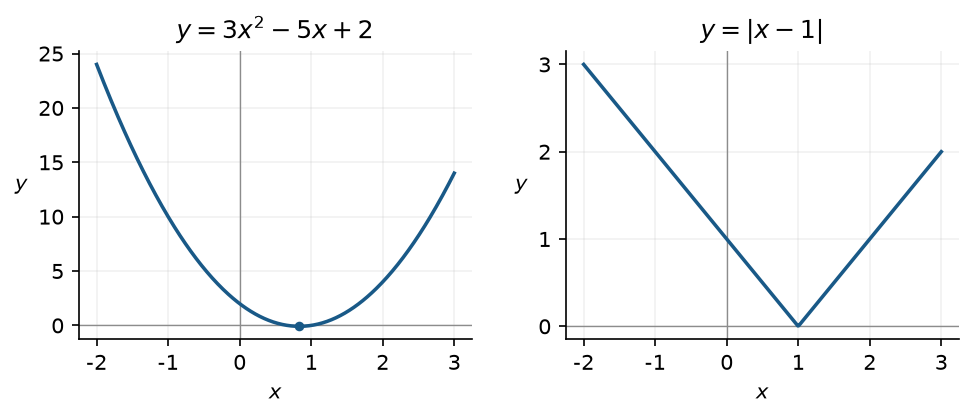
\includegraphics[width=.84\linewidth,height=.38\textheight,keepaspectratio]{figures/C03-HW077-6.png}\end{center}
{\small \field{关联知识}{F04 函数三种表示法、图象与读数（教材帮p.85、86、93、94 / PDF94、95、102、103）；F06 最大值、最小值与值域（教材帮p.99、83、84 / PDF108、92、93）}
\field{方法与易错点}{把关键点与定义域一起标到图上，逐区间读交点和上下关系。 易错：将示意图预测当事实；把两曲线交点收进严格不等式；折线漏端点。}
\field{答案依据}{答案册相关题组：PDF第20、21、22页（册内页19、20、21）；按当前题库原题逐项重算，不按旧版题号机械对套。}}
